\section{Task 2}
% Contents:
% - Introduce the problem
% - Explain why total number is not constant, and choices
% - Explain edge conditions
% - Euler method
% Explain different parts of results, impact of parameters

A well known model for the spread of infectious disease is the SIR-model. The model describes the population at a time t as 
\begin{itemize}
    \item \textbf{Susceptible} S: A person is susceptible if they can get the disease.
    \item \textbf{Infected and infectious} I: A person is infective if they have the disease and can transfer it to others.
    \item \textbf{Removed} R: A person is removed if they can not be infected or infect others.
\end{itemize}

A simple version of SIR-model is
\begin{equation}
    \begin{split}
        \frac{dS}{dt} &= -\beta I S \\
        \frac{dI}{dt} &= \beta IS - \gamma I \\
        \frac{dR}{dt} &= \gamma I. \\
    \end{split}
\end{equation}
Where $\beta$ describes the infectiousness of the model, $\gamma$ describes how quickly the infected become removed.
However, this does not describe the spatial spread of a disease, which can be accommodated for by modifying the equations slightly. One proposed modification is given by Murray \cite{bok}, chapter 13, which is adding
two dispersion terms to account for the spread in space, which gives the following equations
\begin{equation}
    \label{eq:super_sir}
    \begin{split}
        \frac{dS}{dt} &= -\beta I S + \mu_S \Delta S \\
        \frac{dI}{dt} &= \beta IS - \gamma I + \mu_I \Delta I\\
        \frac{dR}{dt} &= \gamma I. \\
    \end{split}
\end{equation}
Where $\mu_S$ and $\mu_I$ describe how much the susceptible and infected move in space. 
Combined with initial values and boundary conditions, this can be solved with numerical schemes.

\subsection{Numerical scheme}
In the following, we further assume that $S(t) + I(t) + R(t) = 1$, so that we are always working with percentages of the total population instead of the actual population.
We consider the case with two spatial dimensions.
To solve the equations we will use the Forward-Euler method, which for (\ref{eq:super_sir}) results in the following scheme
\begin{equation}
    \begin{split}
        S_{n,m}^{l+1} &= S_{n,m}^l + k(-\beta I_{n,m}^l S_{n,m}^l + \mu_S \Delta_h S_{n,m}^l) \\
        I_{n,m}^{l+1} &= I_{n,m}^l + k(\beta I_{n,m}^l S_{n,m}^l - \gamma I_{n,m}^l +  \mu_I \Delta_h I_{n,m}^l) \\
        R_{n,m}^{l+1} &= R_{n,m}^l + k \gamma I_{n,m}^l,  \\
    \end{split}
    \label{eq:SIR-numerical}
\end{equation}
where
\begin{equation*}
    \Delta_h X_{n,m}^l = \frac{1}{h^2}(X_{n+1, m}^l + X_{n-1, m}^l + X_{n, m+1}^l + X_{n, m-1}^l - 4X_{n,m}^l).
\end{equation*}
Here $k$ is the stepsize in time, $h$ the stepsize in both spatial directions and $X$ denotes one of the variables, $S, I$ or $R$. 
$X_{n,m}^l$ corresponds to the numerical solution at $(x_n,y_m,t_l)$. It should be noted that the Forward-Euler scheme is
not stable for all combinations of $h$ and $k$. For the equation $\frac{\partial u}{\partial t} = \alpha \Delta u$, it is stable for all $(h,k)$
such that $\frac{\alpha k}{h^2} < \frac{1}{4}$. This gives a rough estimate for when it is stable for our scheme as well.

We need both initial values and boundary conditions to solve the problem numerically.
The initial values describe the initial distributions of susceptible, infected and recovered people, while
the boundary conditions describe how the different groups move across the boundary of the problem. Since we want the total population to be constant on the domain, we set the boundary conditions to be
\begin{equation}
    \begin{split}
        \nabla S(\partial\Omega) &= \Vec{0} \\
        \nabla I(\partial\Omega) &= \Vec{0} \\
        \nabla R(\partial\Omega) &= \Vec{0}, \\
    \end{split}
\end{equation}
where $\partial\Omega$ is the edge of the domain. 
To discretize this in order $\mathcal{O}(h^2)$, it becomes
\begin{equation}
    \label{eq:num_boundary_task2}
    \begin{split}
        \frac{\Delta_h X_{n,m}^l - \nabla_h X_{n,m}^l}{2h} = 0
    \end{split}
\end{equation}
along the boundaries. Here $\nabla_h$ and $\Delta_h$ operate in $x$ if $n=0$ or $n=N+1$ and in $y$ if $m = 0$ or $m=N+1$, and in both directions where both conditions apply.
To implement this, an extra false boundary is created such that the total grid in space becomes $[-1, N+2] \times [-1, N+2]$. This false boundary will not be part of the model and only used for the numerical solution.
The boundary conditions, equations (\ref{eq:num_boundary_task2}), are then
\begin{equation}
    \begin{split}
        X_{n,-1}^l &= X_{n, 1}^l \\
        X_{n,N+2}^l &= X_{n, N}^l \\
        X_{-1,m}^l &= X_{1, m}^l \\
        X_{N+2,m}^l &= X_{N, m}^l \\
    \end{split}
\end{equation}
on a square grid for $n \in [1, N]$.

\subsection{Results}
As our main exploration we varied both population density and $\beta$ over the grid so we effectively got four areas with different properties. The top
right corner has a high number of infected people, while both the population and $\beta$ is somewhat small. This is the only area where there are infected people in the
beginning. The bottom right corner has a low $\beta$ but a high population, the bottom left has both a high $\beta$ and a high population, and the top left has a high $\beta$ but
a low population.
In figure (\ref{fig:infected-time-evolution}) we can see the time evolution of the infected.
As expected the area with both a high population and high $\beta$ gets infected pretty quickly, while the area with a low $\beta$ remains unaffected for a longer time.
The area with both low population and high $\beta$ gets infected pretty fast, although one can barely see it in the plot. If we look at (\ref{fig:state_10000}), one interesting thing
to note is that some susceptible seem to migrate towards the upper right corner and thereby avoiding the infected somewhat.

\begin{figure}
    \centering
    \begin{subfigure}[b]{0.49\linewidth}
        \centering
        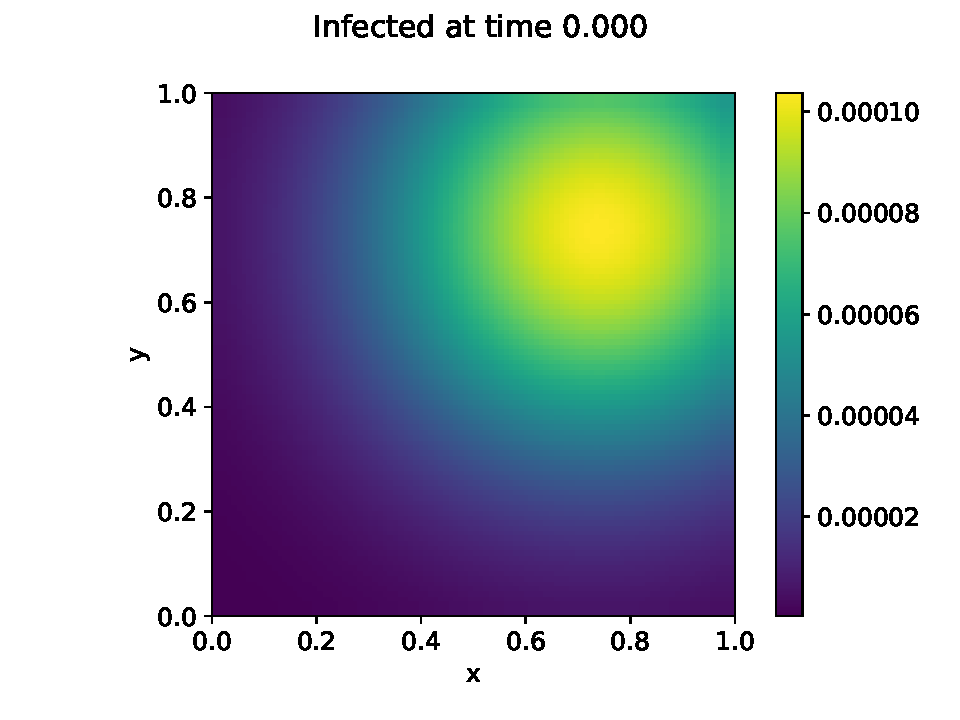
\includegraphics[width=\textwidth]{report/Images/plots/plot-i_t=0-1.pdf}
    \end{subfigure}
    \hfill
    \begin{subfigure}[b]{0.49\linewidth}
        \centering
        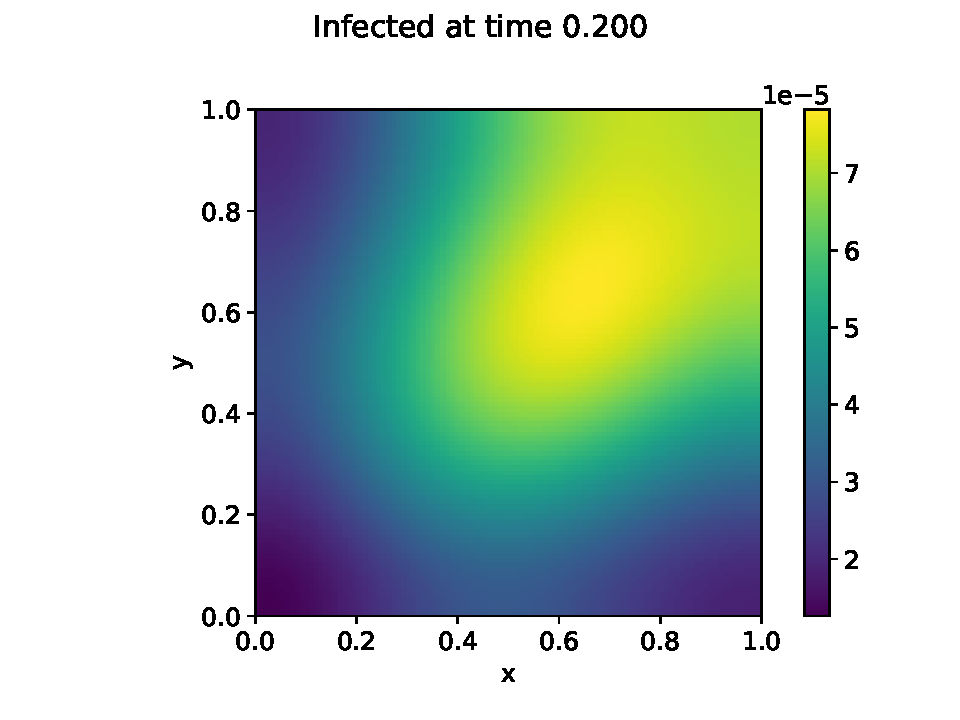
\includegraphics[width=\textwidth]{report/Images/plots/plot-i_t=2000-1.pdf}
    \end{subfigure}
    \begin{subfigure}[b]{0.49\linewidth}
        \centering
        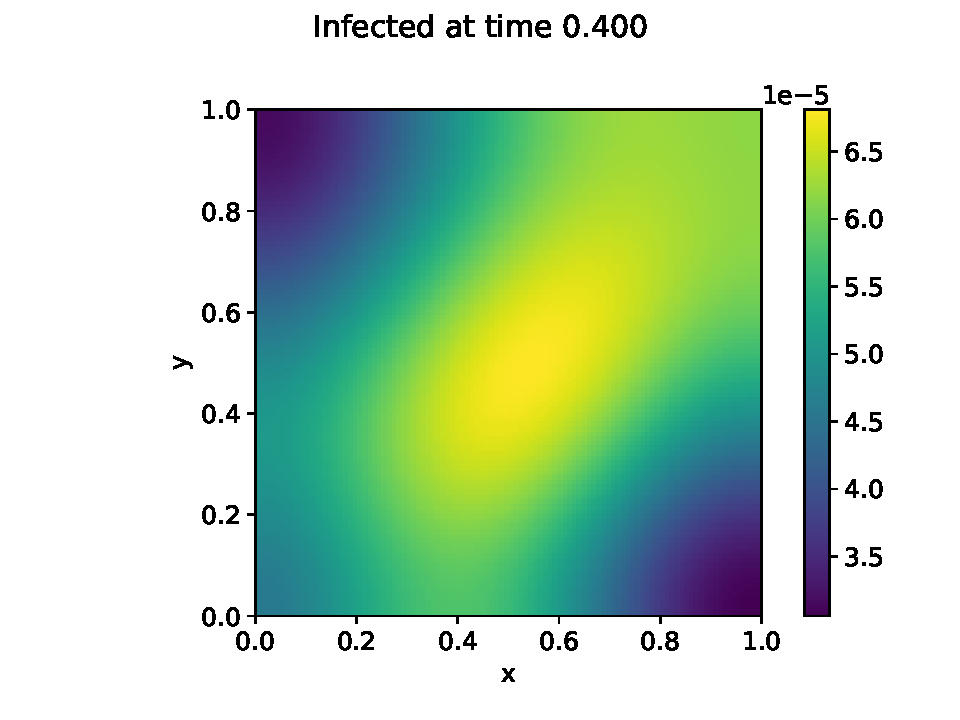
\includegraphics[width=\textwidth]{report/Images/plots/plot-i_t=4000-1.pdf}
    \end{subfigure}
    \hfill
    \begin{subfigure}[b]{0.49\linewidth}
        \centering
        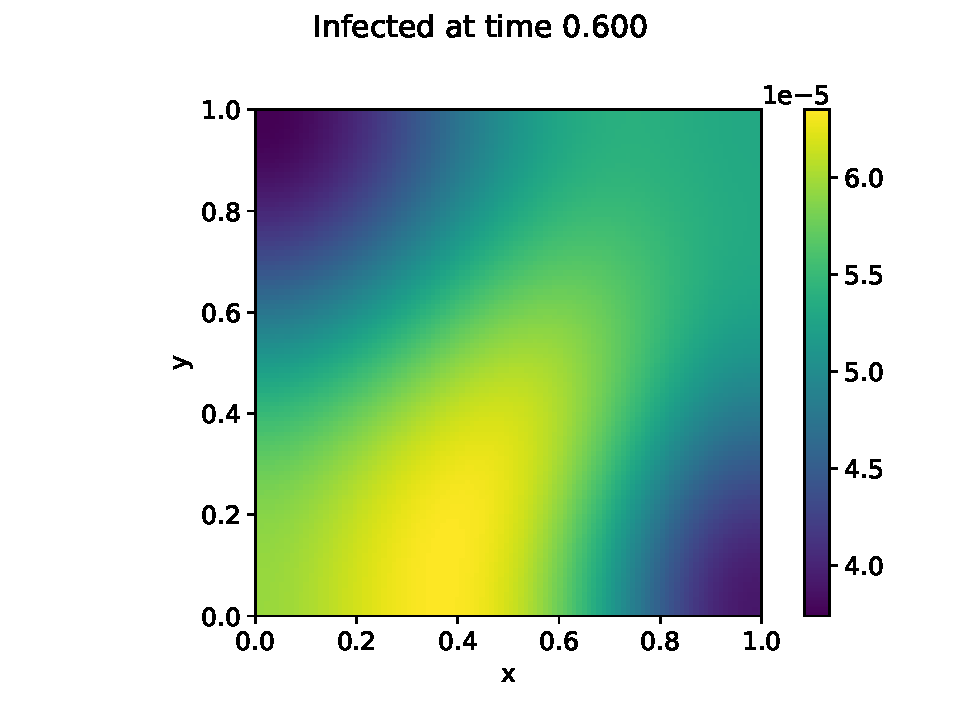
\includegraphics[width=\textwidth]{report/Images/plots/plot-i_t=6000-1.pdf}
    \end{subfigure}
    \hfill
    \begin{subfigure}[b]{0.49\linewidth}
        \centering
        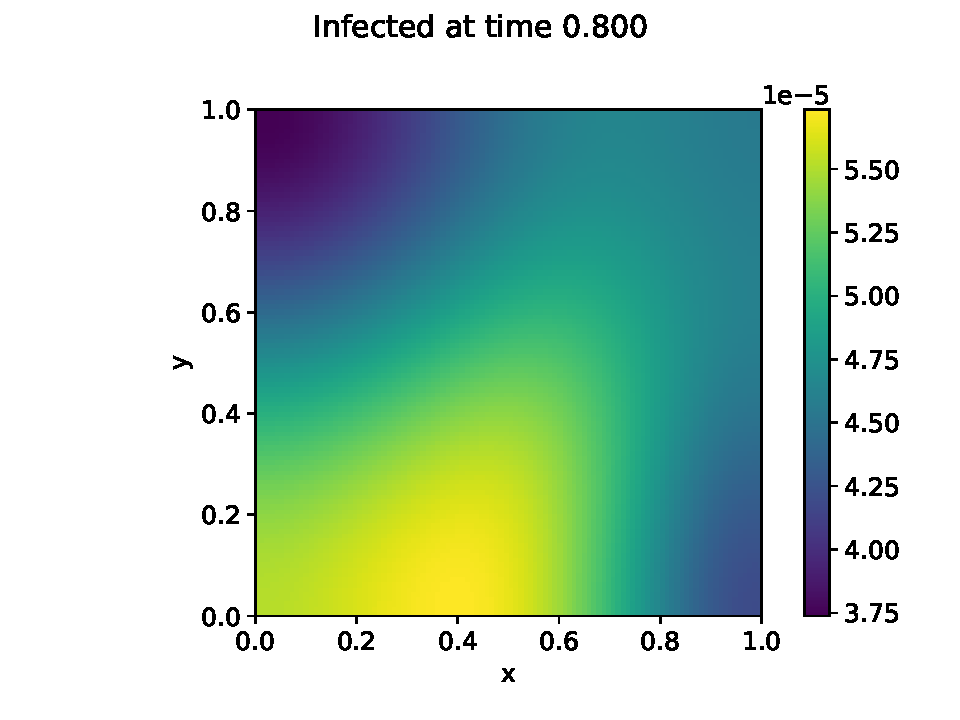
\includegraphics[width=\textwidth]{report/Images/plots/plot-i_t=8000-1.pdf}
    \end{subfigure}
    \hfill
    \begin{subfigure}[b]{0.49\linewidth}
        \centering
        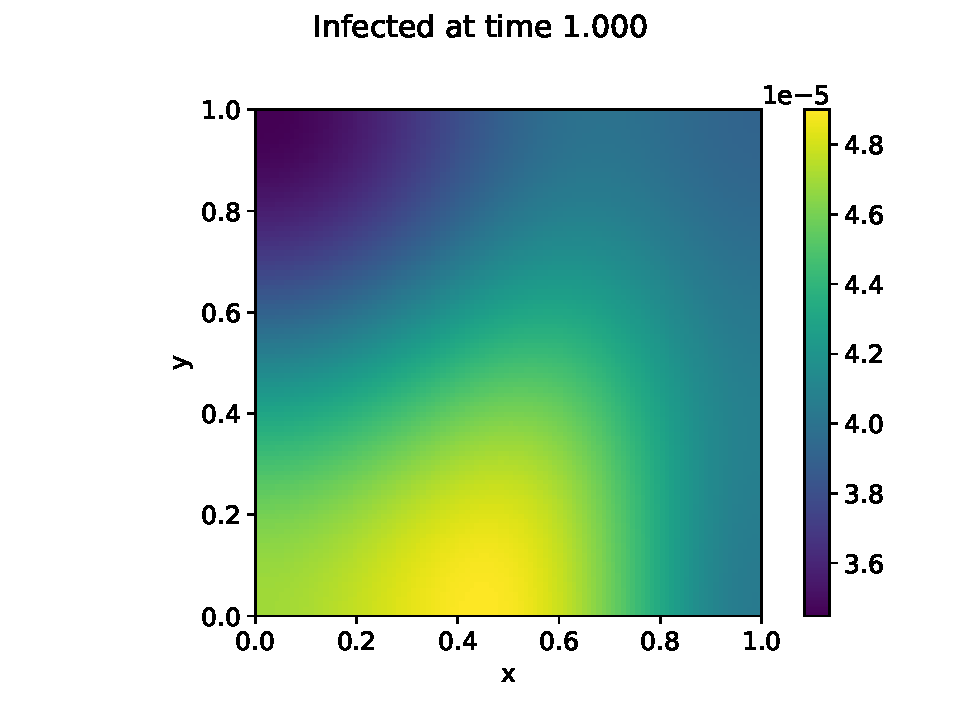
\includegraphics[width=\textwidth]{report/Images/plots/plot-i_t=10000-1.pdf}
    \end{subfigure}
    \caption{Movement of infection areas. The movement of the areas of infection is interesting, not the variation in scaling. $\gamma = 1$, $\mu_I = 0.1$, $\mu_S = 0.1$, $\beta = 100 000 e^{-5((x-0.25)^2 + \frac{(y-0.5)^2}{10})}$.}
    \label{fig:infected-time-evolution}
\end{figure}

\begin{figure}
    \centering
    \begin{subfigure}[b]{0.49\linewidth}
        \centering
        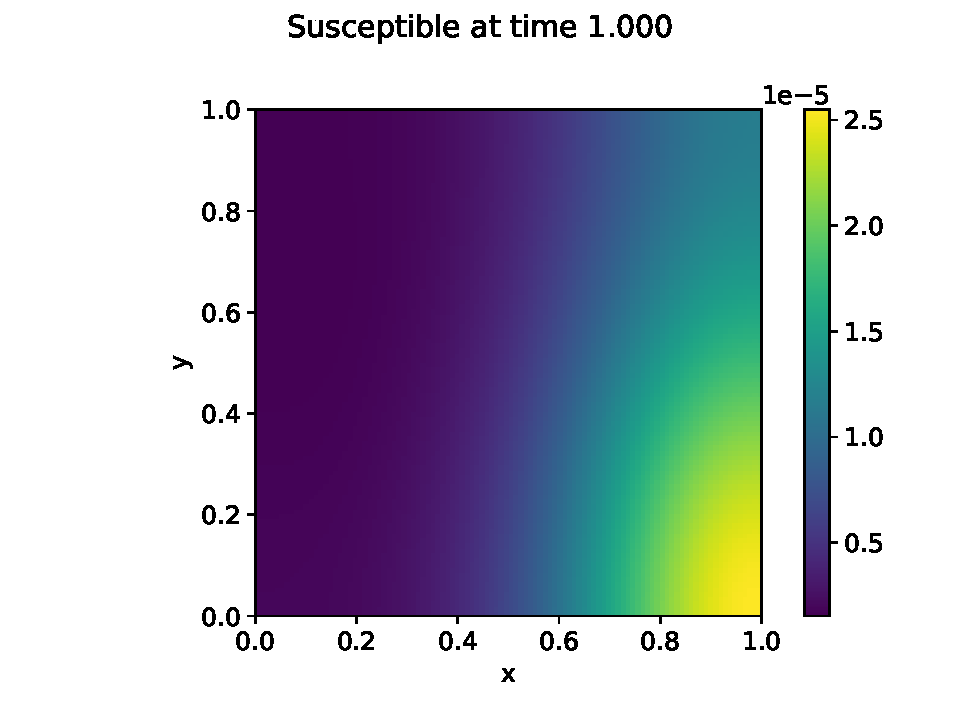
\includegraphics[width=\textwidth]{report/Images/plots/plot-i_t=10000-0.pdf}
    \end{subfigure}
    \hfill
    \begin{subfigure}[b]{0.49\linewidth}
        \centering
        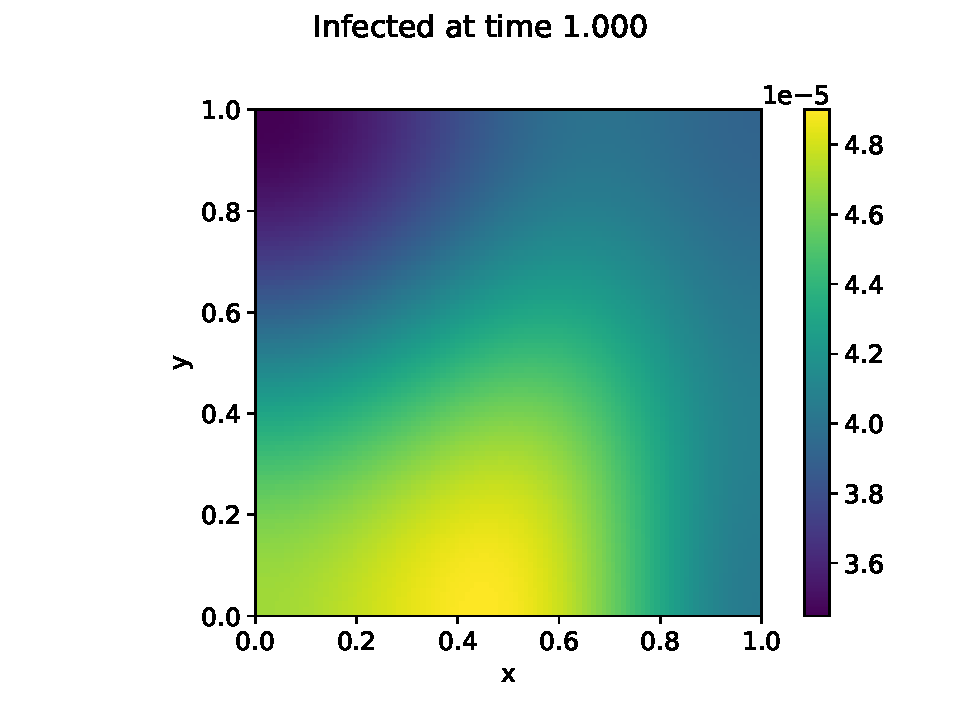
\includegraphics[width=\textwidth]{report/Images/plots/plot-i_t=10000-1.pdf}
    \end{subfigure}
    \hfill
    \begin{subfigure}[b]{0.49\linewidth}
        \centering
        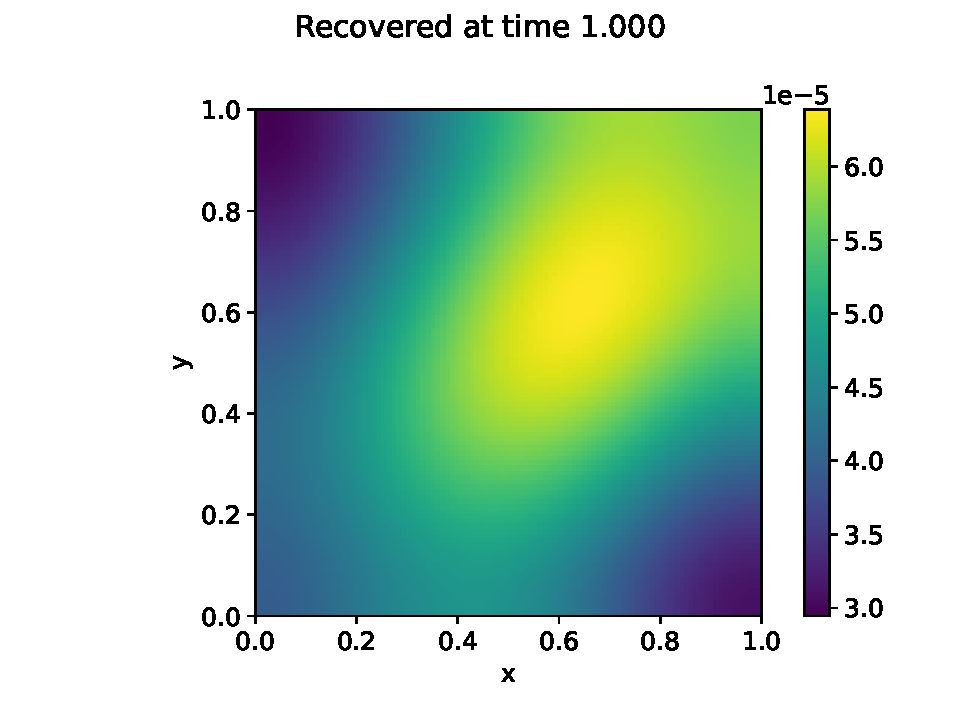
\includegraphics[width=\textwidth]{report/Images/plots/plot-i_t=10000-2.pdf}
    \end{subfigure}
    \caption{Final state of the SIR model. $\gamma = 1,\mu_I = 0.1,\mu_S = 0.1, \beta = 100 000 e^{-5((x-0.25)^2 + \frac{(y-0.5)^2}{10})}$.}
    \label{fig:state_10000}
\end{figure}

Another thing to note is the population size. Although the boundary conditions are set to enforce a constant population size, we still observe a change in population size because of errors in the numerical scheme.
As (\ref{fig:non-constant-population-size}) shows, the population increases slightly during the simulation. 
A possible solution would be to not 
solve for $R(t)$ by equation (\ref{eq:SIR-numerical}) , but rather to let $R(t) = 1- S(t)-I(t)$ such that the total population is constant. This will effectively just 
hide the error in the $R(t)$ term. For this reason we solve the full model as is, and accept an error in the total population size.
\begin{figure}[H]
    \centering
    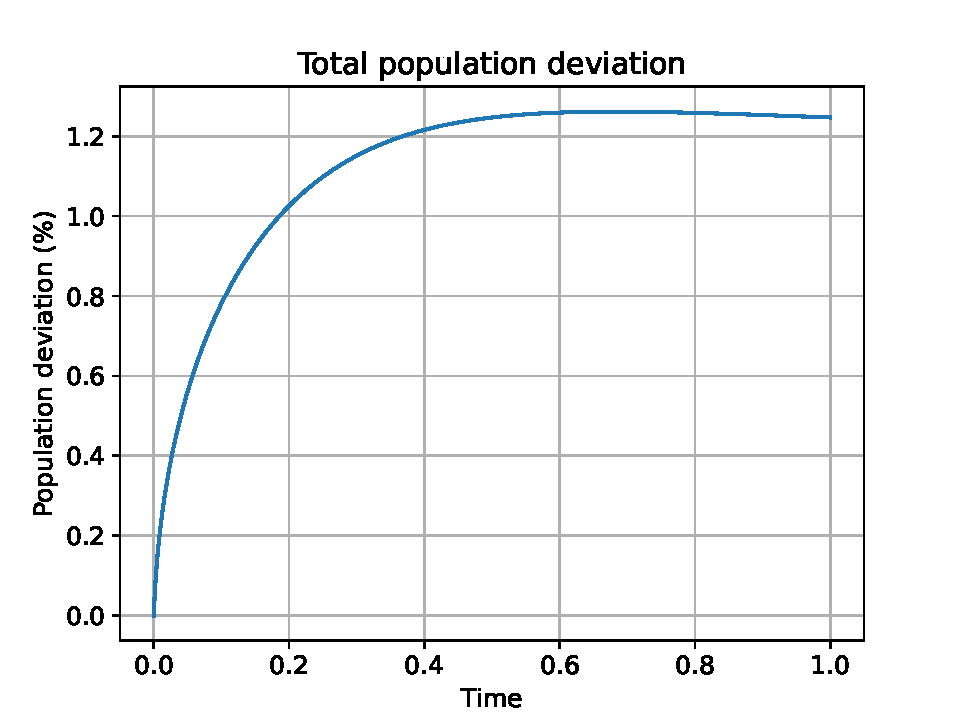
\includegraphics[width=0.5\linewidth]{report/Images/plots/pop_deviation.pdf}
    \caption{The deviation from the standard population we begin with as a function of time.}
    \label{fig:non-constant-population-size}
\end{figure}

The last thing to note is the effect of the parameters on the equation. The size of the spatial domain greatly influences the other 
parameters. The larger domain, the larger the step size in that domain in order to get the same runtime, but that includes larger errors.
In addition, for small stepsizes, the constants such as $\beta$, $\mu_I$, $\mu_S$ need to be larger in order to get the same results.